% mn2esample.tex
%
% v2.1 released 22nd May 2002 (G. Hutton)
%
% The mnsample.tex file has been amended to highlight
% the proper use of LaTeX2e code with the class file
% and using natbib cross-referencing. These changes
% do not reflect the original paper by A. V. Raveendran.
%
% Previous versions of this sample document were
% compatible with the LaTeX 2.09 style file mn.sty
% v1.2 released 5th September 1994 (M. Reed)
% v1.1 released 18th July 1994
% v1.0 released 28th January 1994

\documentclass[useAMS,usenatbib]{mn2e}

% If your system does not have the AMS fonts version 2.0 installed, then
% remove the useAMS option.
%
% useAMS allows you to obtain upright Greek characters.
% e.g. \umu, \upi etc.  See the section on "Upright Greek characters" in
% this guide for further information.
%
% If you are using AMS 2.0 fonts, bold math letters/symbols are available
% at a larger range of sizes for NFSS release 1 and 2 (using \boldmath or
% preferably \bmath).
%
% The usenatbib command allows the use of Patrick Daly's natbib.sty for
% cross-referencing.
%
% If you wish to typeset the paper in Times font (if you do not have the
% PostScript Type 1 Computer Modern fonts you will need to do this to get
% smoother fonts in a PDF file) then uncomment the next line
% \usepackage{Times}

%%%%% AUTHORS - PLACE YOUR OWN MACROS HERE %%%%%
\usepackage{subfigure}
\usepackage{amsmath}	% Advanced maths commands
\usepackage{amssymb}	% Extra maths symbols
\usepackage{graphicx}
\usepackage{algorithm}
\usepackage[noend]{algpseudocode}

\newcommand{\bz}{\bmath{z}}
\newcommand{\bA}{\bmath{A}}
\newcommand{\bB}{\bmath{B}}
\newcommand{\bC}{\bmath{C}}
\newcommand{\bE}{\bmath{E}}
\newcommand{\bF}{\bmath{F}}
\newcommand{\bG}{\bmath{G}}
\newcommand{\br}{\bmath{r}}
\newcommand{\bg}{\bmath{g}}
\newcommand{\bd}{\bmath{d}}
\newcommand{\bv}{\bmath{v}}
\newcommand{\bn}{\bmath{n}}
\newcommand{\by}{\bmath{y}}
\newcommand{\bJ}{\bmath{J}}
\newcommand{\bD}{\bmath{D}}
\newcommand{\bH}{\bmath{H}}
\newcommand{\bN}{\bmath{N}}
\newcommand{\bM}{\bmath{M}}
\newcommand{\bO}{\bmath{O}}
\newcommand{\bP}{\bmath{P}}
\newcommand{\bQ}{\bmath{Q}}
\newcommand{\bR}{\bmath{R}}
\newcommand{\bI}{\bmath{I}}
\newcommand{\ba}{\bmath{a}}
\newcommand{\bb}{\bmath{b}}
\newcommand{\bx}{\bmath{x}}
\newcommand{\bp}{\bmath{p}}
\newcommand{\bmJ}{\bmath{\mathcal{J}}}
\newcommand{\bzero}{\bmath{0}}
%\newcommand{\bvarrho}{\bmath{\varrho}}
%\newcommand{\bnu}{\bmath{\nu}}
%\newcommand{\bvarphi}{\bmath{\varphi}}
\newcommand{\conj}[1]{\overline{#1}}

%%%%%%%%%%%%%%%%%%%%%%%%%%%%%%%%%%%%%%%%%%%%%%%%

\title[Unknown]{TBD}
\author[A. V. Raveendran and A. N. Other]{A. V. Raveendran$^{1}$\thanks{E-mail:
email@address (AVR); otheremail@otheraddress (ANO)} and A. N.
Other$^{2}$\footnotemark[1]\thanks{This file has been amended to
highlight the proper use of \LaTeXe\ code with the class file.
These changes are for illustrative purposes and do not reflect the
original paper by A. V. Raveendran.}\\
$^{1}$Indian Institute of Astrophysics, Bangalore 560034, India\\
$^{2}$Building, Institute, Street Address, City, Code, Country}
\begin{document}

\date{Accepted 1988 December 15. Received 1988 December 14; in original form 1988 October 11}

\pagerange{\pageref{firstpage}--\pageref{lastpage}} \pubyear{2002}

\maketitle

\label{firstpage}

\begin{abstract}
TBD
\end{abstract}

\begin{keywords}
circumstellar matter -- infrared: stars.
\end{keywords}

\section{Introduction}

Main contributions of the paper:

\begin{enumerate}
 \item Present a general framework which unifies all the techniques developed so far showing they are all related (LINCAL, non-linear estimator, etc ...). They are all non-linear
 least-squares techniques, i.e. they either employ Gauss-Newton or the Levenberg-Marquardt algorithms. We have to start with LINCAL showing that it is GN, then we have to motivate 
 why we want to use Oleg's complex optimization framework.
 \item Use Oleg's complex optimization framework to re-derive the non-linear technique proposed by Marthi and Chengular. The novelty lies, in the fact that by using Oleg's
 framework we can find analytic expressions for the Jacobian, the Hessian and the Jacobian-residual product (which is not even the case for LINCAL). State that the algorithm is 
 effectively related to SteFCal and is eff an independent rediscovery of SteFCal and an extension of it into the redundant domain.
 \item Also we present the array geometry function to help us make the derivations from Marthi and Chengular easier to read and understand for a general layout.
 \item We also mention at this point that in Oleg's paper the question is raised is there a fast way of computing the exact inverse, we then present this new method, which is called
 conjugate gradient method. We discuss the algorithm and the two things which bound its execution time. Which is $kappa$ and $m$ (spectral condition number and its sparsity). Then
 we explore both of these parameters.
 \end{enumerate}
 
 **************
 FLOW OF PAPER
 **************
 
 \begin{enumerate}
 \item We need the definition of visibilities as in Liu. DEFINE SNR HERE ALREADY together maybe with the sigma value of the noise.
 \item Introduce the array geometery function.
 \item Write down logcal and lincal in matrix form... ?
 \item Short discussion of least squares and jacobian and hessian's. General GN and LM update rules.
 \item Introduce redundant calibration as a least squares problem. We will use this general fact to derive both popular methods.
 \item Propose a possible solution witch leads to lincal. Mention that this approach works as in this form the function is differentiable (a taylor expansion in the 
 parameters exists). Maybe mention that we can also divide the problem into real and imaginary etc...
 \item Show how this relates to lincal for example ---> show lincal is GN.
 \item Now introduce complex optimization ---> Main motivation for switching to the alternative framework is that the the differentials are very simplistic. We wish to show that
 we can derive the method of Chengular.
 \item Do the derivation of Chengular. 
 \item Brief discussion abouth Chengular and SteFCal and Complex Optimization. Here I show that in Oleg's paper he re-derives an algorithm called SteFCal. Stefcal works
 on the basis of alternating direction implicit method. The first signs of achieving a similar algorithm already appeared in Stefan's conference paper in which the alternating
 idea was first proposed. Then I mention Chegular re-derives the expression by using partial derivatives and extends it to redundant. One could also have used the linear alternating
 approach. In an attempt to merge the terminology that has independently develop in the general calibration and redundant calibration literature and to emphasize the close
 relationship between Stefcal and the approach derived by I will use the label Redunandat SteFCal (R-Stefcal) to refer to the NLS method proposed by ... Lastly we mention that similarly
 to how Oleg re-derived stefcal in, we have achieved the same approach.
 \item Faster Exact inverse. A question that Oleg poses in his paper is, does there exist a faster way to take the exact inverse of JhJ? One that is almost linear, and
 implies that we can therefore implement the full LM algorithm. The aim here is of course to reduce the number of iterations that are required to converge by using the 
 full inverse instead which would hopefully provide enough of a speedup to compensate for the more expensive full-inverse. The algorithm we propose is the conjugate 
 gradient method.
 \item We give the images of the HESSIAN of both lincal and the complex method (number of terms). So we can mention that both are sparse and contain diagonal entries that 
 are more significant than the off-diagonal entries. What linear inversion approach can take advantage of both these phenomenon. One such technique is 
 cg. 
 \item Briefly discuss CG and how its computationally bounded by its condition number and its sparsity (how does the diagonal play a role).
 \item Simulation description
 \item Will CG improve things?
 \item Now first discuss the condition
 number of the Hessian before and after pre-conditioning (pre-codnitioning can only be applied if a good inverse of a matrix is known, if it is known then it can improve 
 the spectral condition number of a matrix. We present here the kappa and iteration number graphs for the HEXAGONAL layout. Although the
 \item Now we discuss the sparsity results. 
 \item Provide a table that theoretical compares R-StEFCal and SPARC.
 \item Number of outerloop iterations. 
 \item Timing results.
 \item Accuracy results.
 \item Maybe some freq simulations.
 \end{enumerate}
 
 We
 
 \section{Visibilities}
The observed visibility $d_{pq}$ measured by the baseline formed by antenna $p$ and $q$ can be described as

\begin{equation}
\label{eq:vis_definition}
d_{pq} = g_{p}\conj{g_q}y_{pq} + n_{pq},
\end{equation}
where $g_{p}$ and $g_{q}$ are the direction independent gains associated with antenna $p$ and $q$, $y_{pq}$ denotes the true visibility that baseline $pq$ measured
and $n_{pq}$ is the thermal noise component. Conjugation is denoted by $\conj{(*)}$. During the course of an actual observation the true value of $g_p$, $g_q$ and $y_{pq}$ are unknown and are the quantities which infact have 
to be estimated.

The real and imaginary components of the thermal noise is normally distributed with a mean of zero and a standard deviation that is equal to [NB - are the real and imaginary parts defined with same sigma?]  
\begin{equation}
\sigma = \frac{\sqrt{2}k_{B}T_{\textrm{sys}}}{A\eta\sqrt{\Delta \nu \tau}}, 
\end{equation}
where $k_B$ is Boltzmann's constant, $T_{\textrm{sys}}$ is equal to the system temperature, $A$ is the effective collecting area of each element in the array, $\eta$ is a dimensionless
efficiency factor, $\Delta \nu$ is the observational bandwidth and $\tau$ is the integration time per visibility. 

\subsection{Redundant Array Geometry Function}
If an array is redundant then its redundant baselines sample the exact same visibilites in the $uv$-plane, i.e. if baseline $pq$ and $rs$ are redundant then $y_{pq} = y_{rs}$. We can
therefore also use the following useful indexing strategy: we can use singular redundant baseline indexes instead of composite antenna pairs to label the true observed visibilities. 

Let $\phi_{ij}:\mathbb{N}^2\rightarrow\mathbb{N}^+$ be the function that maps composite antenna pairs to the unique redundant baseline indexes of an array. We refer to this function 
as the redundant array geometry function in this paper. This mapping is not symmetric as 
$\phi_{ij} = 0$ if $i>j$. We can also define the following symmetric variant of $\phi_{ij}$:
\begin{equation}
\zeta_{ij} = 
\begin{cases}
\phi_{ij}~\textrm{if}~i\leq j\\
\phi_{ji}~\textrm{if}~i>j
\end{cases}.
\end{equation} 
It is possible to construct a simple analytic expression for $\zeta_{ij}$ when our array is in an east-west regular configuration, namely $\zeta_{ij} = |j-i|$. 
It becomes increasingly more difficult to construct analytic expressions of $\zeta_{ij}$ for other more complicated array layouts. The empirically constructed symmetric geometry
functions of three different redundant layouts are depicted in Fig.~\ref{fig:geometry_function}. We denote the range of $\zeta_{ij}$ with $\mathcal{R}(\zeta_{ij})$. The maximal element 
that $\zeta_{ij}$ can ascertain is denoted by $L$ and can be construed as the maximal number of unique redundant baselines which can be formed for a given 
array layout. Alternatively, we can interpret the symmetric geometry functions 
in Fig.~\ref{fig:geometry_function} as matrices. In this alternative paradigm, $\zeta_{ij}$ denotes a matrix entry instead. The dimension of these so called geometry 
matrices are $N\times N$, where $N$ denotes the number of antennas in the array. 

\begin{figure*}
\centering
\subfigure[Hexagonal layout]
{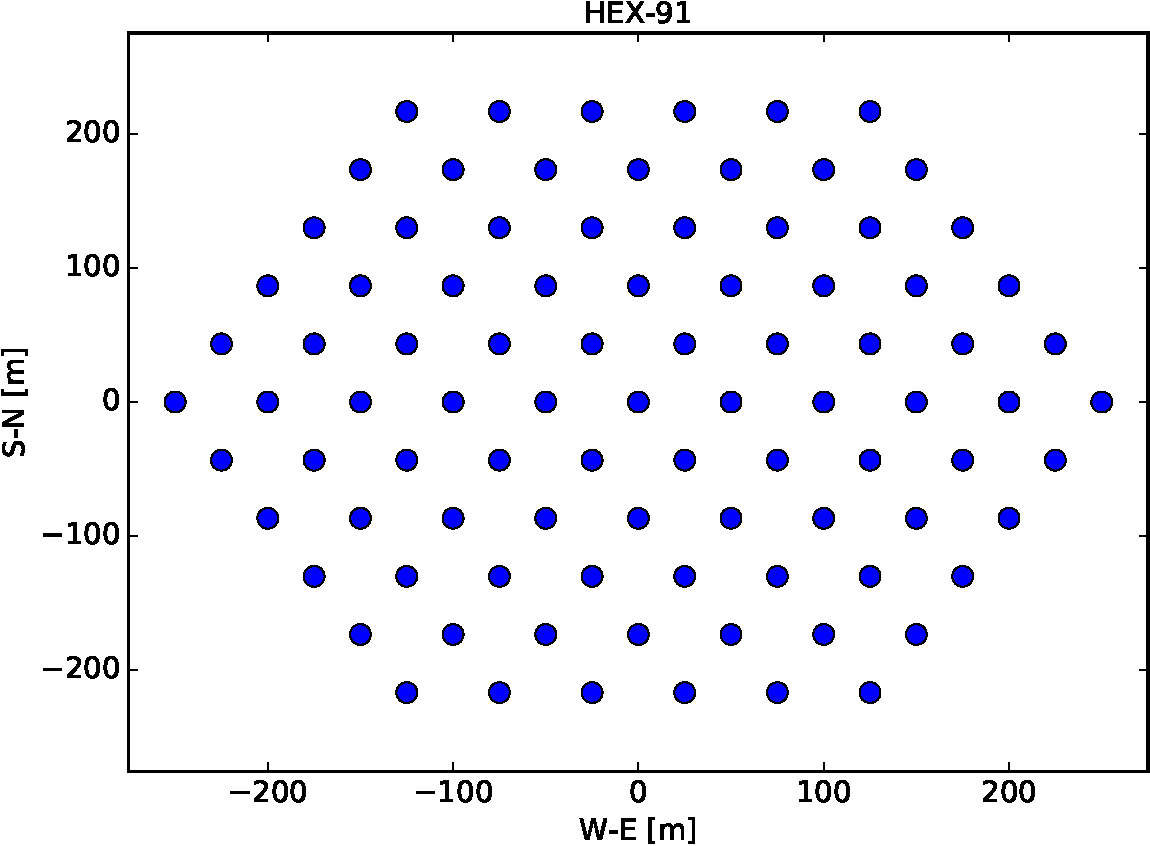
\includegraphics[width=0.33\textwidth]{./HEX_lay.pdf}\label{fig:HEX_lay}}
\subfigure[Square layout]
{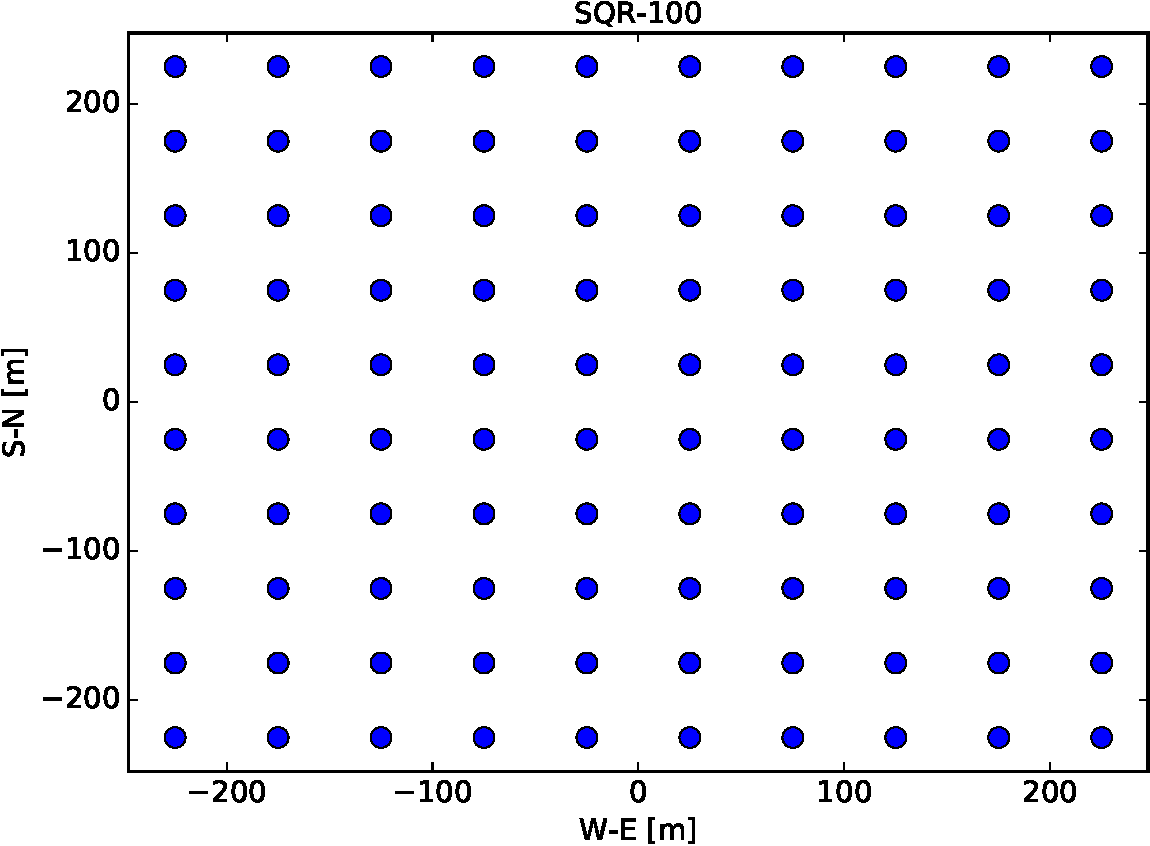
\includegraphics[width=0.33\textwidth]{./SQR_lay.pdf}\label{fig:SQR_lay}}
\subfigure[Regular east-west layout]
{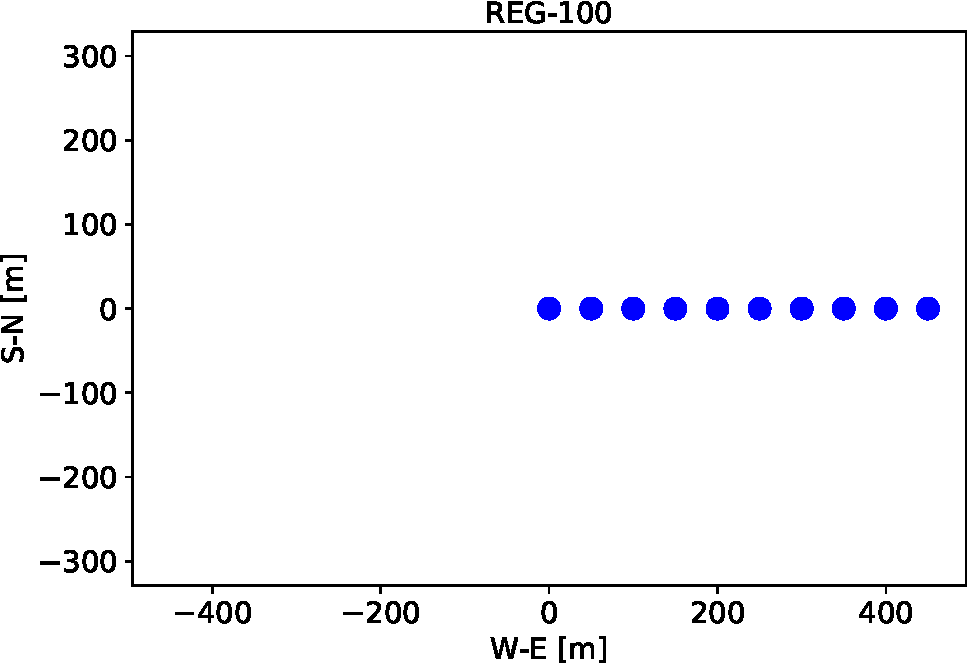
\includegraphics[width=0.33\textwidth]{./REG_lay.pdf}\label{fig:REG_lay}}

\subfigure[Hexagonal: $\zeta_{pq}$]
{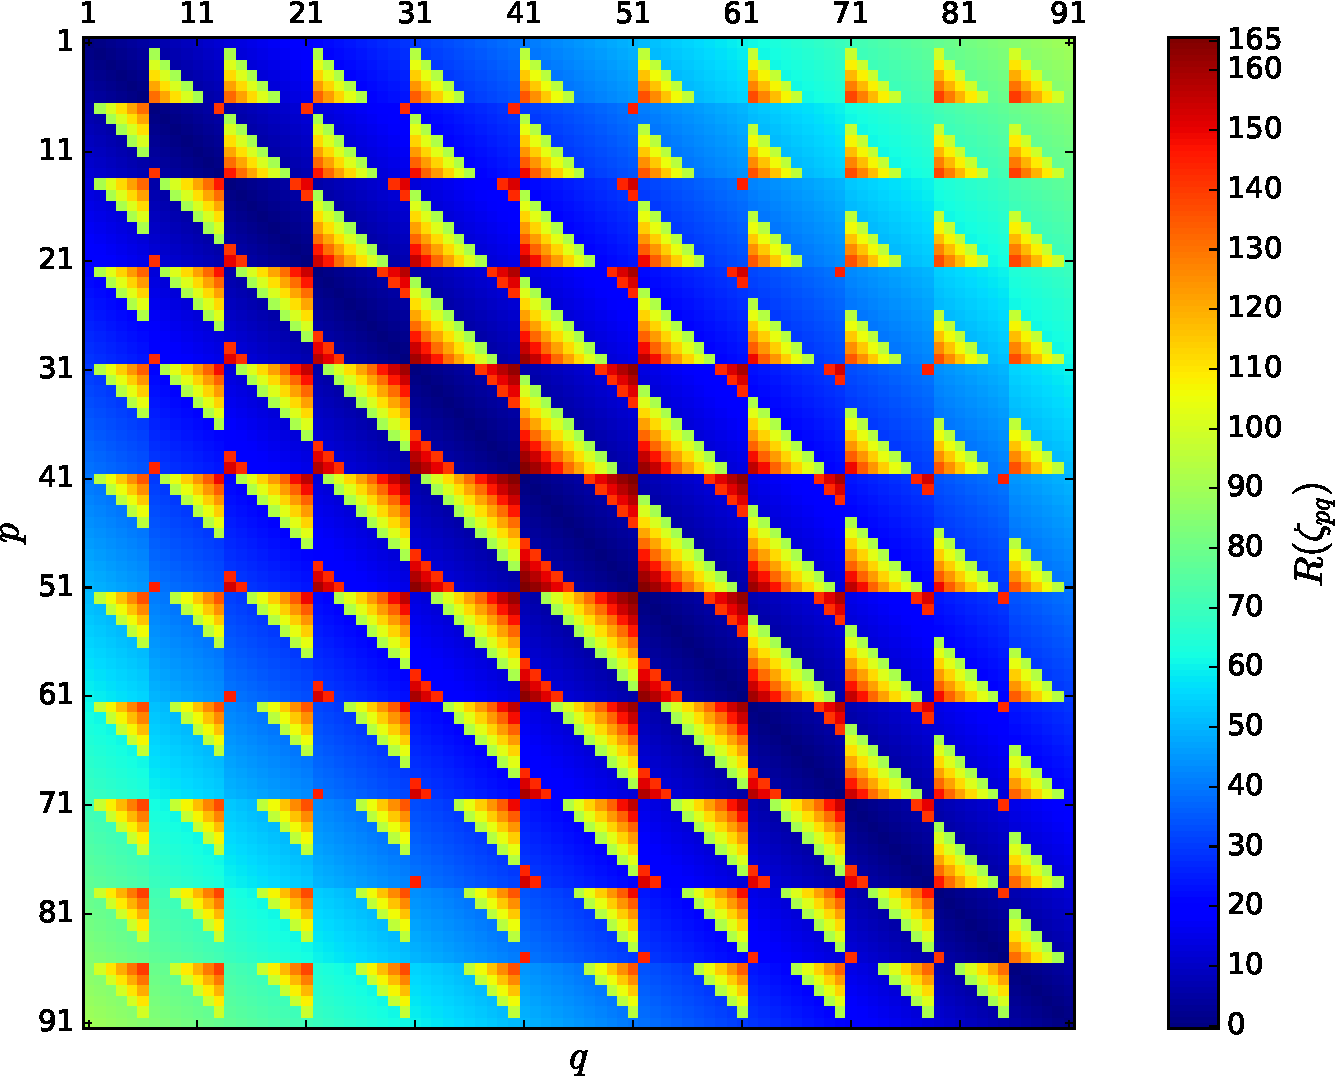
\includegraphics[width=0.33\textwidth]{./HEX_phi.pdf}\label{fig:HEX_phi}}
\subfigure[Square: $\zeta_{pq}$]
{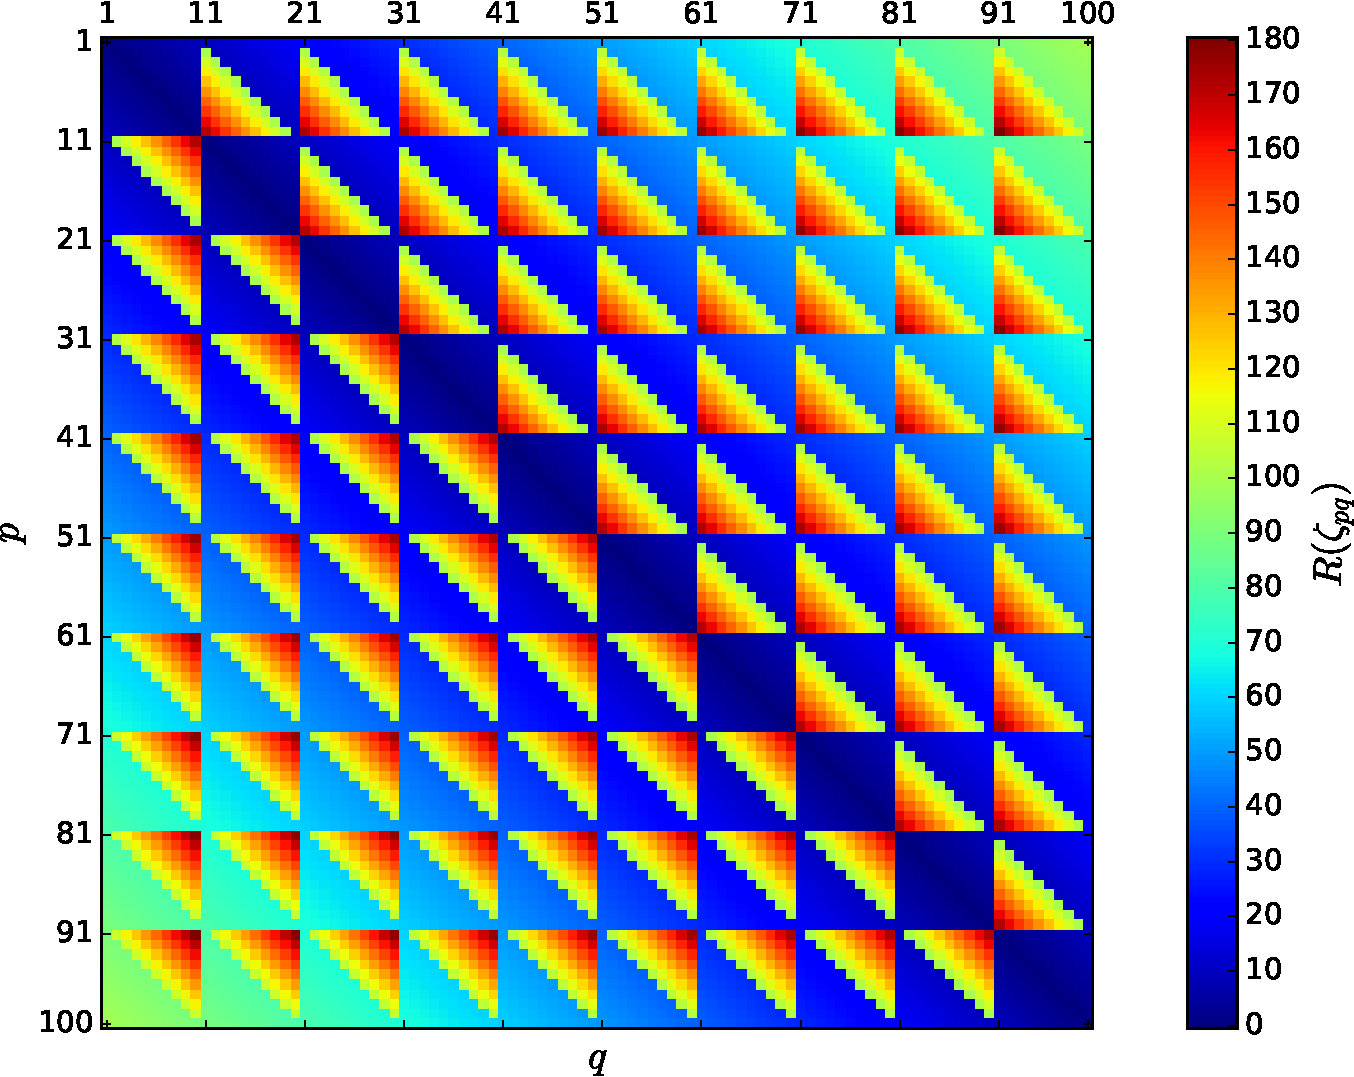
\includegraphics[width=0.33\textwidth]{./SQR_phi.pdf}\label{fig:SQR_phi}}
\subfigure[Regular east-west: $\zeta_{pq}$]
{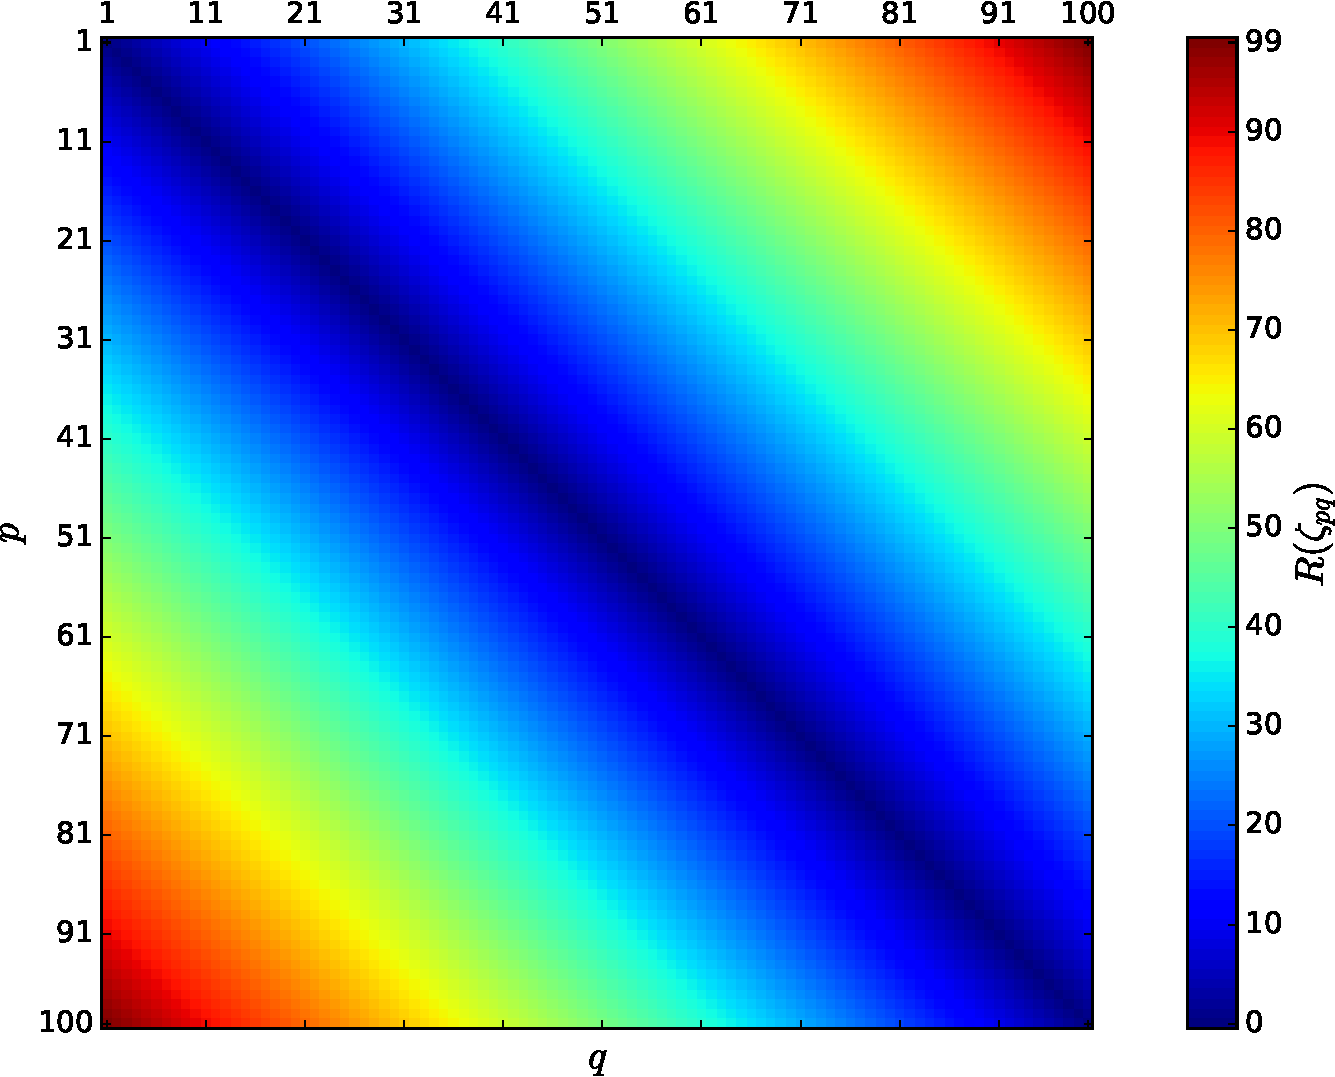
\includegraphics[width=0.33\textwidth]{./REG_phi.pdf}\label{fig:REG_phi}}
\caption{In the top panel we have three different redundant antenna layouts, namely a hexagonal (left), square (middle) and a regular east-west (right) layout. 
In the bottom panel we have the respective symmetric redundancy geometry functions for the layouts on the top panel. We used 91 antennas
to construct the the hexagonal layout, while a 100 antennas where used in the square and east-west layouts. The maximal amount of redundant baselines that can be formed for 
the hexagonal, square and east-west layouts in the top panel are 165, 180 and 99 baselines respectively.\label{fig:geometry_function}}
\end{figure*}

If the function $\phi_{ij}$ is known and one is given one of the two antenna indexes that together form a redundant baseline as well as the redundant baseline index itself then it is possible 
to calculate the unknown antenna index. This can be computed via the following two expressions:
\begin{equation}
\xi_{ij} = 
\begin{cases}
p~\textrm{if}~\exists! ~ p \in \mathbb{N} ~ s.t. ~(\phi_{pi} = j)\\
0~\textrm{otherwise}
\end{cases},
\end{equation}
and
\begin{equation}
\psi_{ij} = 
\begin{cases}
q~\textrm{if}~\exists! ~ q \in \mathbb{N} ~ s.t. ~(\phi_{iq} = j)\\
0~\textrm{otherwise}
\end{cases}
\end{equation}
We use $\xi_{ij}$ to retrieve the first antenna index of the composite antenna pair associated with a particular baseline, if the index of the first antenna in the composite antenna pair and the unique redundant baseline index are known, while we use $\psi_{ij}$ to obtain 
a similar result; the second antenna index of the composite antenna pair. \textbf{NB::} I still need to plot $\zeta_{ij}$ for different antenna layouts.

\subsection{Signal-to-noise Ratio}
If the array is redundant and the function $\phi_{ij}$ is known we can rewrite Eq.~\eqref{eq:vis_definition} as
\begin{equation}
\label{eq:vis_red}
d_{pq} = g_{p}\conj{g_q}y_{\phi_{pq}} + n_{pq}.
\end{equation}
Eq.~\eqref{eq:vis_red} can also be expressed in the following vector form 
\begin{equation}
\label{eq:vis_red_vec}
\bd = \bv + \bn, 
\end{equation}
where 
\begin{align}
 \left [ \bd \right]_{\alpha_{pq}} &= d_{pq}, & \left [ \bv \right ]_{\alpha_{pq}} &= g_p y_{\phi_{pq}} \conj{g_q}\nonumber\\
 \left [ \bn \right ]_{\alpha_{pq}} &= n_{pq}. &  &\label{eq:vec_definitions}
\end{align}
In Eq.~\eqref{eq:vec_definitions}, the size of the three vectors are equal to $B$ (i.e. $p<q$), which denotes the number of baselines in the array. Moreover,
\begin{equation}
\alpha_{pq} =
\begin{cases}
(q-p) + (p-1)\left (N-\frac{1}{2}p \right ) & \textrm{if}~p<q\\
B + (p-q) + (q-1)\left (N-\frac{1}{2}q \right )) & \textrm{if}~p>q\\
%B+q + \frac{1}{2}(p-1)(p-2) & \textrm{if}~p>q\\
0 & \textrm{otherwise}
\end{cases}.
\end{equation}
The easiest way to construct the vectors in Eq.~\ref{eq:vec_definitions} is to enumerate through the composite indexes $pq$ in the following order $12, 13,\cdots,1N,23,\cdots$.
For each composite index we then compute the right hand side of the appropriate vector element definition which we then need to assign to the 
correct vector position. The correct position is calculated with $\alpha_{pq}$. Using the aforementioned order, however, allows you to fill the vector in numerical order, i.e. $12,13,\cdots,1N,23,\cdots \xrightarrow{\alpha_{pq}} 1,2,3,\cdots,B$.  


We will be using the following SNR (signal-to-noise ratio) definition in this paper  
\begin{equation}
\textrm{SNR} = \frac{<\bv\odot\conj{\bv}>_{t,pq}}{<\bn\odot\conj{\bn}>_{t,pq}}, 
\end{equation}
where $<*>_{t,pq}$ denotes averaging over time and baselines and $\odot$ denotes the Hadamard product. The definition we use here is based on the SNR definitions used in \citet{Liu2010} and \citet{Marthi2014}.

\subsection{LOGCAL}
NEED BETTER INTRO\\
One of the best known algorithms that is currently used to perform redundant calibration involves the use of logarithms. If we ignore the noise term then we can 
rewrite Eq.~\eqref{eq:vis_red} as
\begin{eqnarray}
\ln |d_{pq}| &=& \ln |g_p| + \ln |g_q| + \ln |y_{\phi_{pq}}| \label{eq:logcal_amp}\\
\angle d_{pq} &=& \angle g_p - \angle g_q + \angle \phi_{pq} \label{eq:logcal_phase}
\end{eqnarray}

We can easily express Eq.~\eqref{eq:logcal_amp} with the following linear system
\begin{equation}
\widetilde{\bd} = \bA\widetilde{\bz}, 
\end{equation}
where
\begin{equation}
\left [ \widetilde{\bd}\right ]_{\alpha_{pq}} = \ln |d_{pq}|,\nonumber\\ 
\end{equation}
\begin{equation}
\widetilde{\bz} = \begin{bmatrix}
                  \ln | \bg |\\
                  \ln | \by |
                  \end{bmatrix},
\end{equation}
with $\bg = [g_1,g_2,\cdots,g_N]^T$ and $\by = [y_1,y_2,\cdots,y_L]^T$.

Furthermore,
\begin{equation}
\label{eq:A}
\bA = \begin{bmatrix}
       \bA_1 & \bA_2
      \end{bmatrix}
\end{equation}
and
\begin{equation}
\left [ \bA_1 \right ]_{\alpha_{pq},j} = \delta^j_p\vee\delta^j_q,  ~~~ \left [ \bA_2 \right ]_{\alpha_{pq},j} = \delta_{\phi_{pq}}^j. 
\end{equation}

The dimensions of $\bA_1$ and $\bA_2$ are $B\times N$ and $B\times L$.
Moreover, $\vee$ denotes the logical or operator and
\begin{equation}
\delta_y^x  = \begin{cases}
          1 & \textrm{if}~x=y\\
          0 & \textrm{otherwise}
         \end{cases}.
\end{equation}
A similar linear system can be constructed for Eq.~\eqref{eq:logcal_phase}.\\

NEED TO ROUND OF HERE STILL 

\subsection{LINCAL}


\section{Conjugate Gradient Method}
The Conjugate Gradient (CG) method was independently discovered by \citet{Hestenes1973} and \citet{Stiefel1952}. They later published a joint paper, which is now considered as the seminal
reference on CG \citep{Hestenes1952}. The iterative CG method is used to solve a particular class of linear system. The CG method is generally used to solve
\begin{equation}
\label{eq:linear_system}
\bb = \bA\bx,
\end{equation}
where $\bb\in\mathbb{C}^P$ is a known complex column vector of size $P$, $\bx\in\mathbb{C}^P$ is an unknown complex column vector with the same length as $\bb$, and $\bA\in\mathbb{C}^{P\times P}$ is a square positive-definite Hermitian matrix with the appropriate dimensions.  
Moreover, using the CG method to solve Eq.~\eqref{eq:linear_system} will only be computationally advantageous if $\bA$ is also sparse (contain many zero entries).
Using the iterative CG method to solve large sparse linear sytems was popularized by \citet{Reid1971}. A good tutorial on the CG method can be found in \citep{Shewchuk1994}.
The iterative CG method is presented in Algorithm \ref{algo:CG}. 

%If $\bA$ is a square positive semi-definite Hermitian matrix, then the conjugate gradient method only converges if $\bb$ is in the column range of $\bA$ (cite Lu2016).

\begin{algorithm}
\caption{Conjugate Gradient Method. Inputs: $\bA$, $\bb$, a starting value $x$, maximum number of iterations $k_{\textrm{max}}$ and an error tolerance $\epsilon<1$ Output: $\bx$ the solution to Eq.~\eqref{eq:linear_system}. \citep{Shewchuk1994}.}\label{algo:CG}
\begin{algorithmic}[1]
\State $k \gets 0$
\State $\br \gets \bb - \bA\bx$
\State $\bp \gets \br$
\State $\delta_{\textrm{new}} \gets \br^H\br$
\State $\delta_0 \gets \delta_{\textrm{new}}$
\While{$k\leq k_{\textrm{max}}$ and $\delta_{\textrm{new}} > \epsilon^2\delta_0$}
\State $\alpha_k \gets \frac{\delta_{\textrm{new}}}{\bp^H\bA\bp}$
\State $\bx \gets \bx + \alpha_k\bp$
\State $\br \gets \br - \alpha\bA\bp$
\State $\delta_{\textrm{old}} \gets \delta_{\textrm{new}}$ 
\State $\delta_{\textrm{new}} \gets \br^H\br$
\State $\beta_{k} \gets \frac{\delta_{\textrm{new}}}{\delta_{\textrm{old}}}$
\State $\bp \gets \br + \beta\bp$
\State $k \gets k + 1$
\EndWhile
\end{algorithmic}
\end{algorithm}

\subsection{Computational Complexity}
\citet{Kaniel1966} was able to determine convergence bounds for CG using Chebyshev polynomials. A much more in depth analysis of CG convergence can be found in
\citep{Sluis1986}. As can be seen from Algorithm \ref{algo:CG}, the CG method makes use of a major outer loop (line 6 of Algorithm \ref{algo:CG}). It turns out that at worst 
the number of major iterations that CG requires to converge\footnote{If the $\bA$-norm is used to calculate the error.} is proportional to $\sqrt{\kappa}$, where $\kappa$ is the spectral condition number of the matrix $\bA$.
The mathematical definition of $\kappa(\bA)$ is
\begin{equation}
\label{eq:kappa}
\kappa(\bA) = \frac{\lambda_{\textrm{max}}}{\lambda_{\textrm{min}}}, 
\end{equation}
where $\lambda_{\textrm{max}}$ and $\lambda_{\textrm{min}}$ respectively denote the largest and the smallest eigenvalue of $\bA$.
Moreover, the most expensive operation that is conducted within each major loop of Algorithm~\ref{algo:CG} is the vector-matrix product $\bA\bp$, which has a complexity of $\mathbb{O}(m)$, where $m$ is the number of non-zero entries in $\bA$.
The computational complexity of CG is therefore 
\begin{equation}
\label{eq:cg_bound}
\mathbb{O}(\sqrt{\kappa}m). 
\end{equation}
It should now also be clear to the reader why the CG method is especially applicable to sparse linear systems, since in those cases $m < P^2$.

\subsection{Preconditioning}
Preconditioning is a technique which allows us to improve the condition number of a matrix. Let $\bM$ be a positive-definite Hermitian matrix.
We can now indirectly solve for $\bx$ by using 
\begin{equation}
\label{eq:prec}
\bM^{-1}\bA\bx = \bM^{-1}\bb.
\end{equation}
If $\bM$ is a good preconditioner then $\kappa(\bM^{-1}\bA) \ll \kappa(\bA)$, i.e. a good preconditioner lowers the condition number of a matrix which in turn increases the convergence speed 
of CG (see Eq.~\eqref{eq:cg_bound}). The best possible choice of $\bM$ would therefore be $\bA$, which would lead to $\kappa$ (as the largest and smallest eigenvalue of the Identity matrix is equal to one) becoming unity.
If $\kappa$ is one then Eq.~\eqref{eq:cg_bound} simplifies and becomes $\mathbb{O}(m)$. However, if we knew the inverse of $\bA$ then obtaining $\bx$ would be trivial and there would be no need for the CG method in the first place. 
In short, a good preconditioner $\bM$ must approximate $\bA$ fairly accurately. However, if it is not much less expensive to 
compute the inverse of $\bM$ than that of $\bA$ we actually gain nothing (see Eq.~\eqref{eq:prec}).  

If the diagonal entries of $\bA$ is much more significant than its off-diagonal entries then the 
Jacobian preconditioner is a good choice of $\bM$. The Jacobian preconditioner is computed as follows:
\begin{equation}
\bM = \bA\odot\bI, 
\end{equation}
where $\bI$ is the identity matrix. Since the Jacobian preconditioner is a diagonal matrix its inverse can be obtained trivially.

\subsection{Normal Equation}
Lets assume that instead of Eq.~\eqref{eq:linear_system} we have a more general linear system, i.e.
\begin{equation}
 \bb = \bB\bx,
\end{equation}
where $\bb\in\mathbb{C}^K$, $\bx\in\mathbb{C}^P$  and $\bB\in\mathbb{C}^{K \times P}$, with $K > P$. We can use the normal equation 
\begin{equation}
\label{eq:normal_equation}
\bB^H\bB\bx = \bB^H\bb 
\end{equation}
to estimate the $\bx$ that minimizes
\begin{equation}
\label{eq:norm_ls}
\|\bb-\bB\bx\|_F^2. 
\end{equation}
There are a few important observations that we can make while inspecting Eq.~\eqref{eq:normal_equation}:
\begin{enumerate}
\item $\bB^H\bB$ is a square positive semi-definite Hermitian matrix by construction.
\item $\bB^H\bb$ is in the column range of $\bB^H\bB$; this follows trivially from 
\begin{equation}
\bB^H\bb \in \mathcal{R}(\bB^H) \implies \bB^H\bb \in \mathcal{R}(\bB^H\bB).   
\end{equation}
\end{enumerate}

Recall that we mentioned that in general we can only solve Eq.~\eqref{eq:linear_system} with CG if $\bA$ is a square positive-definite Hermitian matrix. The CG method actually has an even broader applicability, it can be used to solve Eq.~\eqref{eq:linear_system} even if $\bA$ is an Hermitian positive semi-definite
square matrix as long as $\bb$ is in the column range of $\bA$ \citep{Lu2015}.

In light of \citet{Lu2015}, the two observations in the numbered list we presented earlier in this section imply that Eq.~\eqref{eq:normal_equation}
can be solved by employing the CG method. The solution returned by CG is however only unique if $\bB^H\bB$ is positive-definite (invertible). The solution
obtained by CG, whether it be unique or not, does however minimize Eq.~\eqref{eq:norm_ls} in a least squares sense.

Note that if $\bA$ is positive semi-definite its smallest eigenvalue is zero, which implies that Eq.~\eqref{eq:kappa} is not defined. \citet{Lu2015} show that when $\bA$
is a square positive semi-definite Hermitian matrix we do not use the spectral condition number to bound the convergence complexity of CG, but the general spectral condition
number instead. The general spectral condition number is very similar to the spectral condition number; the only difference being that in Eq.~\eqref{eq:kappa} we replace  
$\lambda_{\textrm{min}}$ with $\lambda_{\textrm{min}}^+$, which denotes the smallest positive eigenvalue. 

\section{Least Squares}
The method of nonlinear least squares is tanatamount to solving the following optimization problem:  
\begin{equation}
\label{eq:least_squares}
\min_{\bzeta} \Lambda(\bzeta) = \min_{\bzeta} \|\brho\|_F^2 = \min_{\bzeta} \|\bdelta - \bnu(\bzeta)\|_F^2, 
\end{equation}
where $\Lambda$ is known as the objective function, $\brho$ is the residual vector, $\bdelta$ is the observed data vector, $\bnu$ is the model data vector and $\bzeta$ is the solution which minimizes Eq.~\eqref{eq:least_squares}.
The main objective of least squares is to find the model parameters which minimizes the squared difference between the observed data and the model predicted data. Moreover, $\|*\|_F$ denotes the 
Frobenius norm.

The most standard way of solving Eq.~\eqref{eq:least_squares} is to use a gradient type of minimization algorithm. In this paper we will be focusing on the following gradient minimization algorithms: Gauss-Newton and Levenberg-Marquardt \citep{Levenberg1944,Marquardt1963}. 

The gradient based minimization algorithms that are generally used to solve least squares problems generally require the model $\bnu$ to be differentiable
towards each model parameter. When the least squares problem is complex it becomes less straightforward to apply these gradient based minimization methods. The reason being,
many complex functions are not analytic (no Taylor expansion around a fiducial point exists) and therefore not differentiable if the classic notion of differentiation is used. For instance if the 
classical definition of differentiation is used then $\frac{\partial z}{\partial \conj{z}}$, where $z \in \mathbb{C}$, does not exist.

Redundant calibration is achieved by solving the following optimization problem:

The only way to circumvent the differentiability conundrum that plaques complex least square problems is to recast our complex optimization problem in such a way that $\bnu$ becomes analytic in its argument.
The standard way of achieving this is to divide the complex optimization problem into its real and imaginary parts and then to solve for the real and imaginary parts of the parameters separately.

Recently, \citet{Sorber2012} proposed an alternative strategy, which involves the use of Wirtinger calculus \citep{Wirtinger1927}. The Wirtinger derivatives 
are defined to be 
\begin{align}
\label{eq:wir}
\frac{\partial}{\partial z} &= \frac{1}{2}\left ( \frac{\partial}{\partial x} -  i \frac{\partial}{\partial y} \right ),&\frac{\partial}{\partial \conj{z}} &= \frac{1}{2}\left ( \frac{\partial}{\partial x} +  i \frac{\partial}{\partial y} \right ). 
\end{align}
Using the above definitions we can now easily compute the following:
\begin{align}
\frac{\partial z}{\partial z} & = 1, & \frac{\partial \conj{z}}{\partial z}&=0, & \frac{\partial z}{\partial \conj{z}} & = 0, & \frac{\partial \conj{z}}{\partial \conj{z}}&=1.
\end{align}

\subsection{Redundant Calibration}
\citet{Smirnov2015} recently proposed to use this Wirtinger framework instead of the classic real and imaginary approach to perform normal skymodel-based calibration. We will now show
that the Wirtinger framework can also be applied to redundant calibration.

We can perform redundant calibration by solving the following optimization problem: 
\begin{equation}
\label{eq:least_squares_red}
\min_{\bz} \Lambda(\bz) = \min_{\bz} \|\br\|_F^2 = \min_{\bz} \|\bd - \bv(\bz)\|_F^2, 
\end{equation}
where $\bz = [\bg,\by]^T$. The other vectors in Eq.~\eqref{eq:least_squares_red} were defined in Section~\ref{} \footnote{In this paper we use the same symbol to denote corrupted predicted visibilities and true observed corrupted visibilities as it
is trivial to distinguish which one is implied from the context. Using the same symbol for these two quantities improves the readability of the paper.}. Note the similarity between Eq.~\eqref{eq:least_squares} and Eq.~\eqref{eq:least_squares_red},
i.e. redundant calibration can be cast as a non-linear least squares problem. 

Analogous to \cite{Smirnov2015}, we now recast Eq.~\eqref{eq:least_squares_red} to 
\begin{equation}
\label{eq:least_squares_complex}
\min_{\breve{\bz}} \|\breve{\br}\| = \min_{\breve{\bz}} \|\breve{\bd} - \breve{\bv}(\breve{\bz})\|, 
\end{equation}
where $\breve{\bz} = [\bz,\conj{\bz}]^T$, $\breve{\bd} = [\bd,\conj{\bd}]^T$, $\breve{\bv} = [\bv,\conj{\bv}]$. Eq.~\eqref{eq:least_squares_complex} is the augmented counterpart of Eq.~\eqref{eq:least_squares_red}.
If we use the Wirtinger derivatives, Eq.~\eqref{eq:wir}, instead of the classic notion of a derivative to define the gradient operator then 
$\bv$ becomes analytic in $\bz$ and $\conj{\bz}$ as a whole \citep{Smirnov2015}. The fact that $\bv$ is now analytic in its argument has the immediate consequence: it becomes possible to apply complex GN
and complex LM to Eq.~\eqref{eq:least_squares_complex}. 

\subsection{Complex GN and LM}
In this section we discuss how we can use the GN and LM algorithms to solve Eq.~\eqref{eq:least_squares_complex} (i.e. estimate $\breve{\bz}$). The complex Jacobian is defined to be
\begin{equation}
\label{eq:Jacobian}
\bJ = \begin{bmatrix}
       \bmJ & \bmJ^*\\
       \conj{\bmJ}^* & \conj{\bmJ} 
      \end{bmatrix},
\end{equation}
where 
\begin{align}
\bmJ &= \frac{\partial \bv}{\partial \bz}, & \bmJ^* &= \frac{\partial \bv}{\partial \conj{\bz}}. 
\end{align}
In Eq.~\eqref{eq:Jacobian}, $\frac{\partial}{\partial \bz}$ and $\frac{\partial}{\partial \conj{\bz}}$ respectively denote the cogradient operator and the conjugate cogradient operator \citep{Sorber2012}.
The GN update step is now defined as:
\begin{equation}
\label{eq:GN_update}
 \Delta \breve{\bz} = (\bJ^H\bJ)^{-1}\bJ^H\breve{\br}.
\end{equation}
The LM update rule is very similar, the major difference being a damping factor $\lambda$ is introduced:
\begin{equation}
\label{eq:LM_update}
\Delta \breve{\bz} = (\bJ^H\bJ + \lambda\bD)^{-1}\bJ^H\breve{\br},
\end{equation}
where $\bD=\bI\odot\bJ^H\bJ$. 

We use Eq.~\eqref{eq:GN_update} or Eq.~\eqref{eq:LM_update} to iteratively update our 
parameter vector as follows:
\begin{equation}
\label{eq:update}
\breve{\bz}_{k+1} = \breve{\bz}_{k} + \Delta \breve{\bz}_{k}. 
\end{equation}
We update our parameter vector by using Eq.~\eqref{eq:update} until convergence is reached. To improve readability we do not explicitly denote the iteration subscript $k$ in 
Eq.~\eqref{eq:GN_update} and Eq.~\eqref{eq:LM_update}.

\subsection{Analytic Expressions}
If we apply the definition in Eq.~\eqref{eq:Jacobian} to Eq.~\eqref{eq:least_squares_complex} we obtain the following analytic result:
\begin{equation}
\label{eq:Jacobian_red}
\bJ = \begin{bmatrix}
       \bM & \bN\\
       \conj{\bN} & \conj{\bM}
      \end{bmatrix},
\end{equation}
where
\begin{equation}
\bM =\begin{bmatrix}
      \bO & \bP
     \end{bmatrix},
\end{equation}
and 
\begin{equation}
\bN = \begin{bmatrix}
       \bQ & \bzero
      \end{bmatrix}.
\end{equation}
Moreover,
\begin{equation}
\left [ \bO  \right ]_{\alpha_{pq},j} = \begin{cases}
                                         y_{\phi_{pq}}\conj{g_q} & \textrm{if}~p=j\\
                                         0  & \textrm{otherwise} 
                                        \end{cases},
\end{equation}

\begin{equation}
\left [ \bP  \right ]_{\alpha_{pq},j} = \begin{cases}
                                         g_p\conj{g_q} & \textrm{if}~\phi_{pq}=j\\
                                         0  & \textrm{otherwise} 
                                        \end{cases}
\end{equation}
and
\begin{equation}
\left [ \bQ  \right ]_{\alpha_{pq},j} = \begin{cases}
                                         g_py_{\phi_{pq}} & \textrm{if}~q=j\\
                                         0  & \textrm{otherwise} 
                                        \end{cases}
\end{equation}

%\begin{align}
%\left [ \bM_1 \right ]_{\alpha_{pq},j} &= y_{\phi_{pq}}\conj{g_q}\delta_p^j, & \left [ \bM_2 \right ]_{\alpha_{pq},j} &= g_p\conj{g_q}\delta_{\phi_{pq}}^j 
%\end{align}
%\begin{equation}
%\left [ \bN_1 \right ]_{\alpha_{pq},j} = g_py_{\phi_{pq}}\delta^j_q. 
%\end{equation}

It is now trivial to compute the Hessian $\bH$ by using Eq.~\eqref{eq:Jacobian_red}. If we substitute Eq.~\eqref{eq:Jacobian_red} into $\bJ^H\bJ$
we obtain 
\begin{equation}
\label{eq:red_H}
\bH = \bJ^H\bJ = 
\begin{bmatrix}
\bA & \bB\\
\conj{\bB} & \conj{\bA}
\end{bmatrix},
\end{equation}
where

\begin{align}
\bA &= \begin{bmatrix} \bC & \bD\\ \bD^H & \bE \end{bmatrix}, & \bB &= \begin{bmatrix} \bF & \bG\\ \bG^T & \bzero \end{bmatrix},
\end{align}

\begin{equation}
[\bC]_{ij} = 
\begin{cases}
 \sum_{k \neq i} \left | g_k \right |^2 \left | y_{\zeta_{ik}} \right |^2 & \textrm{if} ~ i=j\\
 0 & \textrm{otherwise}
\end{cases},
\end{equation}
\begin{equation}
[\bD]_{ij} = 
\begin{cases}
 g_i \conj{y}_j  \left | g_{\psi_{ij}} \right |^2  & \textrm{if} ~ \psi_{ij}\neq0\\
 0 & \textrm{otherwise}
\end{cases},
\end{equation}

\begin{equation}
[\bE]_{ij} = 
\begin{cases}
 \sum_{pq \in \mathcal{PQ}_i} \left | g_p \right |^2 \left | g_q \right |^2  & \textrm{if} ~ i=j\\
 0 & \textrm{otherwise}
\end{cases},
\end{equation}
\begin{equation}
[\bF]_{ij} = 
\begin{cases}
 g_i g_j  \left | y_{\zeta_{ij}} \right |^2  & \textrm{if} ~ i \neq j\\
 0 & \textrm{otherwise}
\end{cases},
\end{equation}
and
\begin{equation}
[\boldsymbol{G}]_{ij} = 
\begin{cases}
 g_i y_j  \left | g_{\xi_{ij}} \right |^2  & \textrm{if} ~ \xi_{ij}\neq0\\
 0 & \textrm{otherwise}
\end{cases}.
\end{equation}
Moreover, $(*)^T$ denotes matrix transposition and
\begin{equation}
\mathcal{PQ}_i = \left\{pq\in\mathbb{N}^2|(\phi_{pq} = i) \right\}.
\end{equation}

Furthermore, substituting Eq.~\eqref{eq:Jacobian_red} into $\bJ^H\breve{\br}$ results in
\begin{equation}
\bJ^H\breve{\br} = \begin{bmatrix}
                   \ba \\
                   \bb \\
                   \conj{\ba}\\
                   \conj{\bb}
                   \end{bmatrix},
\end{equation}
where
\begin{align}
\label{eq:ab}
\left [ \ba \right ]_i &= \sum_{k\neq i} g_k \widetilde{y}_{ik}r_{ik},  & \left [ \bb \right ]_i &= \sum_{pq\in\mathcal{PQ}_i}\conj{g}_p g_q r_{pq},
\end{align}
and
\begin{equation}
\widetilde{y}_{ik} = 
\begin{cases}
\conj{y}_{\zeta_{ik}} & \textrm{if}~k > i\\
y_{\zeta_{ik}} & \textrm{otherwise}
\end{cases}.
\end{equation}
Moreover $\ba$ and $\bb$ are both column vectors.

HAVE TO RECHECK THE ABOVE EQUATIONS DIRECTLY FROM THE CODE.
DEFINED ALL OPERATORS AND SYMBOLS?

% \begin{equation}
% \boldsymbol{J}^H\breve{\boldsymbol{d}} = 
% \begin{bmatrix}
% \sum_{k\neq i } g_k x_{ik}d_{ik}\\
% \sum_{pq \in \mathcal{I}_j} \conj{g}_p g_q d_{pq}\\
% \downarrow^{*}
% \end{bmatrix}
% \begin{matrix}% matrix for right braces 
% \coolrightbrace{\sum g_k x_{\zeta_{ik}}d_{ik}}{i = 1\cdots N}\\
% \coolrightbrace{\sum \conj{g}_p g_q d_{pq}}{j = 1\cdots L}\\
% \vphantom{\downarrow^{*}}
% \end{matrix}
% \end{equation}



\subsection{Simplifying GN}

The following identities,
\begin{align}
\label{eq:identities}
\frac{1}{3}\bJ\breve{\bz} &= \breve{\bv}, & \bJ^H\breve{\bv} &= \widetilde{\bH}\breve{\bz} 
\end{align}
are trivially established by mechanically showing that the left hand side of each identity in Eq.~\eqref{eq:identities} is equal to its right hand side.
In Eq.~\eqref{eq:identities}, $\widetilde{\bH}$ denotes $\bI\odot\bH$.

Replacing $\breve{\br}$ with $\breve{\bd}-\breve{\bv}$ in Eq.~\eqref{eq:GN_update} results in
\begin{equation}
\label{eq:temp_GN_eq}
\Delta \breve{\bz} = (\bJ^H\bJ)^{-1}\bJ^H(\breve{\bd}-\breve{\bv}), 
\end{equation}
Substituting the first identity of Eq.~\eqref{eq:identities} into Eq.~\eqref{eq:temp_GN_eq} and simplifying the result 
\begin{equation}
\label{eq:one_thrid}
\Delta \breve{\bz} = (\bJ^H\bJ)^{-1}\bJ^H\breve{\bd}-\frac{1}{3}\breve{\bz}.
\end{equation}
It now trivially follows that:
\begin{equation}
\label{eq:two_thrids}
\breve{\bz}_{k+1} = (\bJ^H\bJ)^{-1}\bJ^H\breve{\bd} + \frac{2}{3}\breve{\bz}_{k}. 
\end{equation}
Eq.~\eqref{eq:two_thrids} shows us that in the case of redundant calibration we can calculate the GN update step without calculating the residual. The 
normal skymodel-based equivalent of Eq.~\eqref{eq:two_thrids} is equal to \citep{Smirnov2015}:
\begin{equation}
\label{eq:one_half}
\breve{\bg}_{k+1} = (\bJ^H\bJ)^{-1}\bJ^H\breve{\bd} + \frac{1}{2}\breve{\bg}_{k}, 
\end{equation}
where $\breve{\bg} = [\bg^T,\conj{\bg}^T]^T$

FIX TRANSPOSE PROBLEM

\subsection{GN and LINCAL}
As we mentioned at the start of this section, the Wirtinger framework is not the only way in which we can ensure that $\bv$ is analytic in its argument. We could also 
have divided the problem in Eq ... into its real and imaginary components and then solver for the real and imaginary parts of the parameters separately. There is a third way
of dealing with the issue. We can split the problem in Eq into its phase and amplitude components and then solve for the amplitude and phase of the parameters separately.
This can be achieved by first rewriting Eq. as

\begin{equation}
\label{eq:least_squares_lincal}
\min_{\bmath{\varrho}} \|\breve{\br}\| = \min_{\bmath{\varrho}} \|\breve{\bd} - \breve{\bv}(\bmath{\varrho})\|, 
\end{equation}
where $\bmath{\varrho} = \left [\bmath{\eta},\bmath{\varphi},\widetilde{\bmath{\eta}}, \widetilde{\bmath{\varphi}}\right ]^T$. The Jacobian associated with 
Eq.~\eqref{eq:least_squares_lincal} is equal to the Eq xxx in the LINCAL section.
We have therefore shown that doing one iteration of LINCAL is equivalent to a basic GN update step; the GN update step was just re-derived in the Appendix from first principles.
An easy why of improving the convergence properties of LINCAL would be to simply add the LM damping factor to the basic LINCAL update step. 

\subsection{Diagonalization and StEFCal}
StEFCal (Statistically Efficient Calibration) is an alternating direction implicit method, in which the measurement equation (cite the equation earlier in paper) is linearized by assuming that the gains are known, but
that their conjugates are unknown (REMEMBER TO CITE ALL THE STEFCAL PAPERS MITCHELL ETC...). Under this assumption, the conjugates of the gains can be obtained trivially. Once the conjugates of the gains have been computed, the gains can be solved for. One can then alternate between computing the gains and their conjugates until convergence
is reached. By correctly exploiting the symmetry inherent in the calibration problem this alternating approach can be replaced by a single iterative update step [MUST IMPROVE HERE]. \cite{Salvini2014} also show that
the convergence of the algorithm can be improved if for every even iteration the basic update step is modified as follows: the current gain estimate is replaced by the average of the current gain solution and the gain solution of the previous odd iteration.
StEFCal lowers the computational complexity of normal skymodel-based calibration from O$(P^3)$ to O$(P^2)$. 

\citet{Smirnov2015} recently showed that one can also derive StEFCal by viewing normal skymodel-based calibration as a complex optimization problem. They first compute the skymodel-based calibration equivalent analytic expressions of $\bJ$,
$\bH$ and $\bJ^H\breve{\br}$. While inspecting the skymodel-based $\bH$ it becomes apparent that its diagonal entries are much more significant than its off-diagonal entries.
By approximating $\bH$ by its diagonal and substituting this approximate Hessian back into the GN update step they are able to re-derive the fundamental StEFCal update step. They then show that the 
averaging update step used on even iterations can be derived by substituting the approximate $H$ into the LM update step, whilst setting $\lambda$ to one.

The natural question now arises: is it possible to derive a redundant calibration variant of the SteFCal algorithm if we follow a similar approach to what \citet{Smirnov2015}
proposed?

Inspecting Eq.~\eqref{eq:red_H} reveals that in the case of redundant calibration the Hessian's diagonal entries are also more significant than its off-diagonal entries.
If we substitute $\bJ^H\bJ$ with $\widetilde{\bH}$ (by its diagonal approximation) and replace $\breve{\br}$ with $\breve{\bd} - \breve{\bv}$ in Eq.~\eqref{eq:GN_update} we obtain
\begin{equation}
\label{eq:appr_GN}
 \Delta \breve{\bz} \approx \widetilde{\bH}^{-1}\bJ^H(\breve{\bd}-\breve{\bv})
\end{equation}
Utilizing the second identity in Eq.~\eqref{eq:identities} allows us to simplify Eq.~\eqref{eq:appr_GN} to
\begin{equation}
  \Delta \breve{\bz} \approx \widetilde{\bH}^{-1}\bJ^H\breve{\bd}-\breve{\bz}.
\end{equation}
It now trivially follows that
\begin{equation}
 \breve{\bz}_{k+1} \approx \widetilde{\bH}^{-1}\bJ^H\breve{\bd}.
\end{equation}
We obtain a similar result if we repeat the above procedure, only in this case we use Eq.~\eqref{eq:LM_update} instead,
namely
\begin{align}
\breve{\bz}_{k+1} &\approx \frac{1}{1+\lambda}\widetilde{\bH}^{-1}\bJ^H\breve{\bd} + \frac{\lambda}{1+\lambda} \breve{\bz}_k,\label{eq:lambda}\\
 &= \alpha \widetilde{\bH}^{-1}\bJ^H\breve{\bd} + (1-\alpha)\breve{\bz}_k, \label{eq:alpha}  
\end{align}
where $\alpha = \frac{1}{1+\lambda}$. Moreover, $\lambda = \frac{1-\alpha}{\alpha}$. The analytic expression of $\bJ^H\breve{\bd}$ will be very similar to the analytic 
expression of $\bJ^H\breve{\br}$, the only difference being that in Eq.~\eqref{eq:ab} the letter $r$ would be replaced by a $d$. If we substitute the analytic expression
of $\bJ^H\breve{\bd}$ and $\widetilde{\bH}^{-1}$ (which is easily computed as the matrix is a diagonal matrix) into Eq.~\eqref{eq:alpha} we obtain the following two update rules:
\begin{equation}
\label{eq:g_update}
g_{i}^{k+1} = \alpha \frac{\sum_{j\neq i} g_j^k \widetilde{y}_{ij}^{~\!\!k} d_{ij}}{\sum_{j\neq i} |g_j^k|^2|y_{\zeta_{ij}}^k|^2} + (1-\alpha) g_i^k, 
\end{equation}
and
\begin{equation}
\label{eq:y_update}
y_{i}^{k+1} = \alpha \frac{\sum_{pq \in \mathcal{PQ}_i} \conj{g}_p^k g_q^k d_{pq}}{\sum_{pq \in \mathcal{PQ}_i}|g_p^k|^2|g_q^k|^2} + (1-\alpha) y_i^k. 
\end{equation}

The question now arises what value should we use for $\alpha$? Although an exact mathematical proof for the optimal choice of $\alpha$ still eludes us, it is still possible to
venture a clever guess by studying what the choice of $\alpha$ is in the case of StEFCal. The StEFCal equivalent of Eq.~\eqref{eq:two_thrids}
is equal to
\begin{equation}
\label{eq:one_half}
\breve{\bg}_{k+1} = (\bJ^H\bJ)^{-1}\bJ^H\breve{\bd} + \frac{1}{2}\breve{\bg}_{k}. 
\end{equation}
Note that in Eq.~\eqref{eq:one_half} the influence that the estimate of the parameters from the previous iteration has on the current iteration is scaled by a half, while
in Eq.~\eqref{eq:two_thrids} it is scaled by two thirds. Moreover, the StEFCal equivalent of Eq.~\eqref{eq:lambda} and Eq.~\eqref{eq:alpha} are
\begin{align}
\breve{\bg}_{k+1} &\approx \frac{1}{1+\lambda}\widetilde{\bH}^{-1}\bJ^H\breve{\bd} + \frac{\lambda}{1+\lambda} \breve{\bg}_k,\label{eq:stef_lambda}\\
 &= \alpha \widetilde{\bH}^{-1}\bJ^H\breve{\bd} + (1-\alpha)\breve{\bg}_k, \label{eq:stef_alpha}  
\end{align}

On the odd iterations $\lambda$ is chosen to be zero, which corresponds to an $\alpha$ equal to one. On the even iteration $\lambda$ is chosen to be equal to one, which corresponds
to an $\alpha$ equal to a half. Note that, on the odd iteration the influence that the estimate of the parameters of the previous iteration has on the current estimate is scaled
by a half. Which is exactly the same as in, Eq.~\eqref{eq:one_half}.  

If we wish to scale $\breve{\bz}$ by two thirds in Eq.~\eqref{eq:alpha} we should choose $\alpha$ equal to a third, which corresponds to a $\lambda$ equal to two.

At this point there is no way of knowing if this is mere coincidence. DEF REWRITE THIS.

REWRTIE THIS IN A DIFFERENT WAY. START WITH CHENGULAR AND JUST MENTION THE LINK TO STEFCAL'S CHOICE OF ALPHA.

The update rules in Eq.~\eqref{eq:lambda} and Eq.~\eqref{eq:alpha} have been derived before, by Chengular... The approach they followed is discussed in the Appendix.

Interestingly enough, if we substitute $\alpha = 1$ into Eq.~\ref{eq:g_update} then it reduces to the skymodel-based StEFCal update rule. In Chengular they propose 
an $\alpha = 0.3$.

In an attempt to merge the terminology that has independently develop in the general calibration and redundant calibration literature and to emphasize the close
relationship between Stefcal and the approach derived by I will use the label Redunandat SteFCal (R-Stefcal) to refer to the NLS method proposed by ... 

****\\

with $\alpha = \frac{1}{1+\lambda}$. Moreover $\lambda = \frac{1-\alpha}{\alpha}$. So in Marthi and Chengular (2014) they use an $\alpha$ of 0.3, which corresponds to an LM damping factor $\lambda$
of $2\frac{1}{3}$.

























% fiducial initial guess 
% 
% The following partial derivatives are now easily computed
% 
% \begin{eqnarray}
% \frac{c_{ij}}{\partial \eta_p} &=& y_{i-j} e^{\eta_p - i \varphi_p} e^{\eta_q - i \varphi_q}\\ 
% \frac{c_{ij}}{\partial \varphi_p} &=&  -i y_{i-j} e^{\eta_p - i \varphi_p} e^{\eta_q - i \varphi_q}\\
% \frac{c_{ij}}{\partial \eta_q} &=& y_{i-j} e^{\eta_p - i \varphi_p} e^{\eta_q - i \varphi_q}\\ 
% \frac{c_{ij}}{\partial \varphi_q} &=&  i y_{i-j} e^{\eta_p - i \varphi_p} e^{\eta_q - i \varphi_q}\\
% \frac{y_{i-j}}{\partial \varphi_q} &=&  e^{\eta_p - i \varphi_p} e^{\eta_q - i \varphi_q}
% \end{eqnarray}
% 
% 
% The Wirtinger derivative is used in the last equation.
% 
% \begin{eqnarray}
% c_{ij} &\approx& c_{ij}^0 + \Delta \eta_p(y_{i-j}^0 e^{\eta_p^0 - i \varphi_p^0} e^{\eta_q^0 - i \varphi_q^0}) + \Delta \eta_q(y_{i-j}^0 e^{\eta_p^0 - i \varphi_p^0} e^{\eta_q^0 - i \varphi_q^0})\\
% && -i\Delta\varphi_p (y_{i-j}^0e^{\eta_p^0 - i \varphi_p^0} e^{\eta_q^0 - i \varphi_q^0}) +i\Delta\varphi_q (y_{i-j}^0e^{\eta_p^0 - i \varphi_p^0} e^{\eta_q^0 - i \varphi_q^0})\\
% && y_{i-j}^1(y_{i-j}^0e^{\eta_p^0 - i \varphi_p^0} e^{\eta_q^0 - i \varphi_q^0})\\
% &\approx&  c_{ij}^0 + e^{\eta_p^0 - i \varphi_p^0} e^{\eta_q^0 - i \varphi_q^0}(y_{i-j}^1 + y_{i-j}^0( \Delta \eta_p+ \Delta \eta_q - i\Delta\varphi_p + i\Delta\varphi_p))
% \end{eqnarray}
% 
% \begin{equation}
% \label{eq:residual}
% r_{ij} = \delta_{ij} = c_{ij}-c_{ij}^0 = e^{\eta_p^0 - i \varphi_p^0} e^{\eta_q^0 - i \varphi_q^0}(y_{i-j}^1 + y_{i-j}^0( \Delta \eta_p+ \Delta \eta_q - i\Delta\varphi_p + i\Delta\varphi_p)) 
% \end{equation}
% 
% Eq.~\ref{eq:residual} allows us to construct the following linear system:
% 
% \begin{equation}
% \boldsymbol{J}[\boldsymbol{\Delta \eta},\boldsymbol{\Delta \varphi},\boldsymbol{\Delta y}]^T = \boldsymbol{r}, 
% \end{equation}
% 
% where $\boldsymbol{J}$ is equal to 
% \begin{equation}
% \boldsymbol{J} = \bigg [\overbrace{\frac{c_{pq}}{\partial \eta_p}}^{i= 1\cdots N},~\overbrace{\frac{c_{pq}}{\partial \varphi_p}}^{i= 1\cdots N},~\overbrace{\frac{c_{pq}}{\partial y_{t}}}^{t=1\cdots r_s} \bigg ] \bigg \} [pq] = 1\cdots N_{\textrm{b}} (p<q) 
% \end{equation}
% or
% \begin{equation}
% \boldsymbol{J} = \bigg [\frac{c_{pq}}{\partial \boldsymbol{\eta}},~\frac{c_{pq}}{\partial \boldsymbol{\varphi}},~\frac{c_{pq}}{\partial \boldsymbol{y}} \bigg ] \bigg \} [pq] = 1\cdots N_{\textrm{b}} (p<q). 
% \end{equation}
% 
% The last column is again a Wirtinger derivative.
% 
% Which means we can obtain the least-squares estimate as follows:
% 
% \begin{equation}
% [\boldsymbol{\Delta \eta},\boldsymbol{\Delta \varphi},\boldsymbol{\Delta y}]^T = [\boldsymbol{J}^H\boldsymbol{J}]^{-1}\boldsymbol{J}^H\boldsymbol{r}.
% \end{equation}




\bibliographystyle{mn2e}
\bibliography{paper}

\appendix

\section{LINCAL}
In this section we derive LINCAL \citep{Liu2010} from first principles.
%Assume that $\eta_p,\eta_q,\widetilde{\eta}_{\phi_{pq}},\varphi_p,\varphi_q$ and $\widetilde{\varphi}_{\phi_{pq}}$ are real valued variables.
We can rewrite Eq.~\eqref{eq:vis_red_vec} to
\begin{equation}
\label{eq:lincal_vec}
\bd = \bv(\bvarrho) + \bn, 
\end{equation}
where 
\begin{align}
\left [ \bv(\bvarrho) \right ]_{\alpha_{pq}} &= e^{\eta_p - i \varphi_p} e^{\widetilde{\eta}_{\phi_{pq}}- i \widetilde{\varphi}_{\phi_{pq}}} e^{\eta_q + i \varphi_q}\\
&= v_{pq},
\end{align}
and
\begin{equation}
\bvarrho = 
\begin{bmatrix}
\bmath{\eta} \\
\bvarphi \\
\widetilde{\bmath{\eta}} \\
\widetilde{\bvarphi}
\end{bmatrix},\qquad
\begin{aligned}
\bmath{\eta} &= [\eta_1, \eta_2,\cdots \eta_N]^T\\
 \bmath{\varphi} &= [\varphi_1, \varphi_2,\cdots \varphi_N]^T\\
 \widetilde{\bmath{\eta}} &= [\widetilde{\eta_1}, \widetilde{\eta_2},\cdots \widetilde{\eta_L}]^T\\
 \widetilde{\bmath{\varphi}} &= [\widetilde{\varphi_1}, \widetilde{\varphi_2},\cdots \widetilde{\varphi_L}]^T
\end{aligned}.
\label{eq:help}
\end{equation}
Note that the vectors $\bmath{\eta},~\bvarphi,~\widetilde{\bmath{\eta}}$ and $\widetilde{\bvarphi}$ are real valued.

The first order Taylor expansion of Eq.~\eqref{eq:lincal_vec} around the fiducial point $\bvarrho_0$ is equal to
\begin{equation}
\label{eq:d_lin}
\bd = \bv_0 + \bmJ_0 \Delta \bvarrho  + \bn.
\end{equation}
If we calculate the residual, dropping the reference to a specific fiducial point, we obtain: 
\begin{equation}
\label{eq:r_lin}
\br = \bd - \bv = \bmJ \Delta \bvarrho + \bn.
\end{equation}
Moreover,
\begin{equation}
\label{eq:jac_upper_lincal}
\bmJ = \begin{bmatrix}
       \bN & \bM 
       \end{bmatrix},
\end{equation}
where
\begin{align}
\bN &= \begin{bmatrix} \bO & \bP \end{bmatrix}, & \bM &= \begin{bmatrix} \bQ & \bR \end{bmatrix}, 
\end{align}
\begin{equation}
 [\bO]_{\alpha_{pq},j} =  \frac{\partial v_{pq}}{\partial \eta_j} = \begin{cases} 
    v_{pq} &\textrm{if}~(p=j)~\textrm{or}~(q=j)\\
    0 & \textrm{otherwise}
   \end{cases},
\end{equation}
\begin{equation}
 [\bP]_{\alpha_{pq},j} =  \frac{\partial v_{pq}}{\partial \varphi_j} = \begin{cases}
                                                                        i v_{pq} &\textrm{if}~ p=j\\
                                                                        -i v_{pq} &\textrm{if}~ q=j \\
                                                                        0 & \textrm{otherwise} 
                                                                       \end{cases}
\end{equation}
\begin{equation}
 [\bQ]_{\alpha_{pq},j} =  \frac{\partial v_{pq}}{\partial \widetilde{\eta}_j} = \begin{cases} 
    v_{pq} &\textrm{if}~\phi_{pq}=j\\
    0 & \textrm{otherwise}
   \end{cases},
\end{equation}
\begin{equation}
 [\bR]_{\alpha_{pq},j} =  \frac{\partial v_{pq}}{\partial \widetilde{\varphi}_j} = \begin{cases} 
    i v_{pq} &\textrm{if}~\phi_{pq}=j\\
    0 & \textrm{otherwise}
   \end{cases}.
\end{equation}
Augmenting the residual by taking into account its conjugate results in 
\begin{equation}
\breve{\br} = \bJ \Delta \bvarrho + \bn, 
\end{equation}
where $\breve{\br} = \begin{bmatrix}\br^T & \conj{\br}^T \end{bmatrix}^T$ and 
\begin{equation}
\bJ = 
\begin{bmatrix}
 \bmJ\\  
 \conj{\bmJ}
\end{bmatrix}.
\end{equation}
The solution to 
\begin{equation}
 \min_{\Delta \bvarrho} \| \breve{\br} - \bJ \Delta \bvarrho\|_F^2,
\end{equation}
is equal to 
\begin{equation}
\label{eq:LINCAL_update}
\Delta \bvarrho = (\bJ^H\bJ)^{-1} \bJ^H\breve{\br}. 
\end{equation}
Eq.~\eqref{eq:LINCAL_update} is used to iteratively determine a new estimate of the parameter vector $\bvarrho$ as follows
\begin{equation}
\label{eq:new_rho}
\bvarrho_{k+1} = \bvarrho_k + \Delta \bvarrho_k. 
\end{equation}
Note that we do not explicitly denote the $k$ index in Eq.~\eqref{eq:LINCAL_update}. We update our parameter vector until convergence is reached.   
\label{lastpage}
\end{document}
